\section{Property-Driven Development}
\label{sec:pdd}

In order to work with the PDD methodology in practice, it is important that the system-level designer and the RT-level designer understand the required steps (as shown in Figure~\ref{fig:PDD-overview}) in more detail.
The first step is the refinement and analysis of the system-level model, after which the properties are generated and, lastly, the hardware is designed.
Step one and two are automatically executed by \textit{SCAM}. 
Therefore, in the following, we provide a basic idea of what happens insides DeSCAM. 
The last step is explained by an example.

\subsection{Step 1: Model analysis}
\label{sec:model-analysis}

\begin{wrapfigure}{l}{0.3\textwidth}
	\vspace{-20pt}
    \caption{Parsing and analysing}
    \label{fig:step1-detail}
    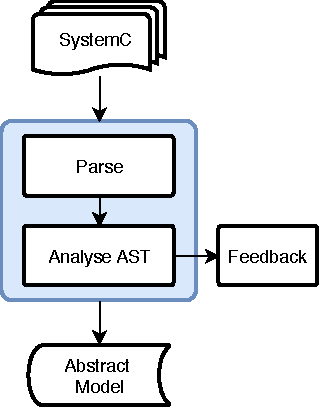
\includegraphics[width=0.3\textwidth]{fig/step1_detail}
    \vspace{-40pt}
\end{wrapfigure}

The refinement and analysis of the SystemC model is divided into two intermediate steps as shown in Figure~\ref{fig:step1-detail}.
The model is parsed and analyzed for compliance with the SystemC-PPA subset.
Then, structural and behavioral information is extracted and stored in an internal data structure referred as abstract model (AM).
If the designer uses statements that are not part of the subset, warnings are generated and the model has to be refined accordingly. 

\subsubsection{Parsing and Analysing}

In this step, the SystemC model is parsed by the open source compiler llvm/clang, as explained in \cite{2013-KaushikPatel}.
The main reason for using \textit{clang} is that the resulting abstract-syntax-tree (\href{https://en.wikipedia.org/wiki/Abstract_syntax_tree}{AST}) implements a design pattern called \href{https://en.wikipedia.org/wiki/Visitor_pattern}{visitor pattern}. 
An AST stores program code in a tree-like structure and contains all static information related to the program, for example the SystemC scheduler.
The combination of the AST and the visitor pattern enables an efficient analysis of the object structure.

Next, the AST is analyzed and all information that is required for property generation is extracted. 
In a nutshell: All C++ specific details, for example the SystemC scheduler, are stripped away and only information that is required to describe a module in terms of structure and behavior is stored in the AM. 
The structural information (e.g., ports and variables) are stored as an AST and the behavior (described by the thread) is stored in form of a control flow graph (blockCFG).

\begin{wrapfigure}{l}{0.3\textwidth}
	\vspace{-10pt}
    \caption{blockCFG translation}
    \label{fig:step2-detail}
    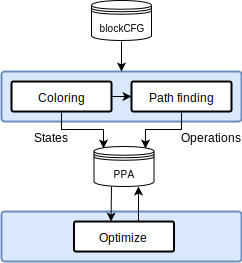
\includegraphics[width=0.3\textwidth]{fig/step2_detail}
    \vspace{-20pt}
\end{wrapfigure}

The tool analyzes each object of the C++ program and checks for compliance with SystemC-PPA. 
If an object violates this SystemC subset, feedback in form of warnings and errors is generated and the objects are not stored in the AM.
\textbf{Important:} The designer has to check the errors/warnings before implementing the RTL.
It is possible, that the absence of objects in the AM alters the behavior described by the SystemC design. 

For example, the line ``\textit{std::cout \textless\textless ``Hello" \textless\textless std::endl}" produces the error ``\textit{-E- Unknown error: Stmts can't be processed(d)}". 
There are two possibilities for dealing with such an error. 
First, the designer is sure that std::cout pipes to the console. 
In this case the error is negligible. 
Second, the standard behavior of \textit{std::cout} is changed and e.g., the stream pipes to a variable, which has an effect on the behavior of the module. 
In this case the design behavior is different in absence of the statement. 
The designer has to refine the SystemC description to match the subset, otherwise the generated properties are meaningless. 

The code for parsing and analyzing can be found in \textit{src/ParseSystemC} and the abstract model is described in \textit{src/Model}.  
The class \textit{src/ParseSystemC/ModelFactory} is the core element for creating the abstract model. 
The user is granted access to the AM by writing a backend.
A detailed description on writing your own backend is found in \textit{src/Backend/}. 

\subsubsection{blockCFG translation}

A major benefit of the PDD methodolgy is that a sound relationship between a system-level model and a RTL implementation is established. 
From a mathematical point of view, the relationship is sound with respect to LTL properties. This implies that any LTL property proven on the abstract model will also hold on the RTL model. 
From a practical point of view, any design property shown to hold on the system level will also hold on the RTL. 
Hence, the task of system verification can be moved from the RTL to the system level and the result will translate automatically to the RTL. 

After parsing and analyzing the system-level model the behavior is stored as a blockCFG.
In order to ensure soundness an explicit representation of the I/O behavior is required. However, the provided blockCFG describes the behavior in terms of the control flow and contains the I/O behavior only implicitly.
The blockCFG therefore has to be transformed to a different graph, which describes the I/O behavior as a PPA.
The PPA has an important state for each call to a communication interface at the system level and a state transition for each possible execution path between two calls (referred to as \textit{operation}).  

Figure~\ref{fig:step2-detail} shows a schematic overview of the transformation flow from a blockCFG to a PPA.
The transformation is separated into two steps: \textit{Coloring} involves finding the important states and \textit{path finding} elaborates execution paths between two important states on the blockCFG.
The PPA is then optimized regarding size and complexity, described by the \textit{optimization} step. 


For explaining the details of the transformation the example of Figure~\ref{fig:system-c-example-complex} is used. 
The module describes a framer hardware that searches for the start of a data frame. 
This behavior is described in the section \textit{idle}.
As long as no new frame is detected the hardware stays in the section \textit{idle}. 
After the detection of a new frame a shared output is set to \textit{true} and the module changes to section start. 
The module stays in this state until the \textit{master\_out} port did send the messages 3, 2, and 1. 
Then, the module switches to the section \textit{frame\_data} and reads 15 frames. 
After completion the module goes back to the section \textit{idle} and waits for the start of a new message. 


\begin{wrapfigure}{r}{0.5\textwidth}
  \centering  
  \begin{minipage}{0.9\linewidth}
    \sffamily\small
    \begin{tabbing}
99 \= XXX\=XXX\=XXX\=XXX\=XXX\=XXX\=XXX\=\kill
1:\' enum status\_t \{in\_frame, oof\_frame\};\\
2:\' struct msg\_t \{status\_t status; int data; \};\\
3:\' SC\_MODULE(Example) \{ \\
4:\'\> SC\_CTOR(Example): \\
5:\'\>\> nextsection(idle)\{SC\_THREAD(fsm)\}; \\
6:\'\> enum Sections\{idle,frame\_start,frame\_data\}; \\
7:\'\> Sections section,nextsection; \\
8:\'\> blocking\_in$<$msg\_t$>$ b\_in; \\
9:\'\> master\_out$<$int$>$m\_out; \\
10:\'\> shared\_out$<$bool$>$ s\_out; \\
11:\'\> int cnt;bool ready;msg\_t msg; \\
12:\'\> void fsm()\{ \\
13:\'\>\> while(true) \{ \\
14:\'\>\>\> section = nextsection; \\
15:\'\>\>\> if(section == idle)\{ \\
16:\'\>\>\>\> s\_out$\rightarrow$set(false); \\
17:\'\>\>\>\> b\_in$\rightarrow$read(msg);\\
18:\'\>\>\>\> if(msg.status == in\_frame)\{\\
19:\'\>\>\>\>\> s\_out$\rightarrow$set(true); \\
20:\'\>\>\>\>\> nextsection = frame\_start;\\
21:\'\>\>\>\>\> cnt = 3;\\
22:\'\>\>\>\> \}\\
23:\'\>\>\> \}else if(section == frame\_start)\{ \\
24:\'\>\>\>\> m\_out$\rightarrow$write(cnt);\\
25:\'\>\>\>\> cnt = cnt-1;\\
26:\'\>\>\>\> if (cnt == 0) \{\\
27:\'\>\>\>\>\> cnt = 15;\\
28:\'\>\>\>\>\> nextsection = frame\_data;\\
29:\'\>\>\>\> \}\\
30:\'\>\>\> \}else if(section == frame\_data)\{ \\
31:\'\>\>\>\> ready = b\_in$\rightarrow$nb\_read(msg);\\
32:\'\>\>\>\> if (!ready) \{ \\
33:\'\>\>\>\>\> m\_out$\rightarrow$write(msg.data);\\
34:\'\>\>\>\>\> if(cnt == 0)\{nextsection = idle;\}\\
35:\'\>\>\>\>\> cnt = cnt-1;\\
36:\'\>\>\>\> \}\\
37:\'\>\>\> \}\\
38:\'\>\> \}\}\};\\
    \end{tabbing}
  \end{minipage}
  
  \caption{SystemC-PPA example}
  \label{fig:system-c-example-complex}
\end{wrapfigure}



The transformation requires several intermediate steps.
The result of the first intermediate step is shown in Figure~\ref{fig:cfg_colored}.
Each node represents a line in the source code, e.g., \textit{L.16} stands for the line~16 in Figure~\ref{fig:system-c-example-complex}, which is the first statement executed after reset. 
Execution continues with \textit{L.17} and afterwards \textit{L.18}.
This statement is an if-then-else statement and if the condition evaluates to \textit{false}, the section remains the same and execution continues with execution of \textit{L.16}. 
This results in an edge from \textit{L.18} to \textit{L.16}. 
If the condition evaluates to \textit{true} the execution continues with \textit{L.19}.

The blockCFG of Figure~\ref{fig:cfg_colored} is obtained from the blockCFG of the thread \textit{fsm()} provided by clang in step~\ref{sec:model-analysis}.
It is known that the thread is SystemC-PPA compliant and thereby follows a specific structure.
Thus, it is possible to simplify the blockCFG by removing the \emph{while(true) loop}, the \emph{if-then-else} for the sections and the \emph{nextsection} assignment (if present).
If such a node is removed from the graph, each incoming edge is merged with each outgoing edge. 
For example, the node for line~20 is removed from the blockCFG and \textit{L.21} is redirected to the first statement of section \textit{frame\_start}.

Removing the \textit{nextsection} assignment of line~34 is more difficult. 
After \textit{L.34} is evaluated \textit{L.35} is executed. 
The successor of \textit{L.35} is dependent on the evaluation of \textit{L.34}. 
If \textit{L.34} evaluates to \textit{true} execution continues with section \textit{idle}, otherwise \textit{frame\_data}. 
This problem is solved, as shown in Figure~\ref{fig:cfg_colored}, by duplicating node \textit{L.35} and connecting each instance to a distinct section \textit{start}. 

\subsubsection{Coloring and Path finding}

The nodes that are marked red in Figure~\ref{fig:cfg_colored} indicate a communication call. 
Initially the coloring is unknown and in order to find the communication calls the graph is searched. 
Here, we are only interested in calls that implement a synchronization.
The respective nodes are marked and transformed to a state for the PPA. 

\begin{wrapfigure}{r}{0.25\textwidth}
			\vspace{-20pt}
		\caption{Operation P2}
		\label{fig:example_operation}
		\begin{small}
		\begin{lstlisting}
assume:
 state == L.17 and
 sync == true and 	
 msg.status==in_frame;
prove: 
 state == L.24
 s_out == true;
 cnt == 3;
\end{lstlisting}
\end{small}
\end{wrapfigure}

Now, all possible paths between two communication states are computed.
Each path results in a property, which checks the correct transitioning between two I/O states at the RTL. 
In this way, it is ensured that the hardware shows the same I/O behavior as the system-level.

Properties are described as interval properties and are checked by the means of interval property checking (IPC) on the RTL design. 
A property has assumptions and expectations. 
If the assumptions are true (the operation \textit{triggers}) the property checker proves or disproves the expectations. 

For example, in state \textit{L.17} there are two outgoing paths \textit{P1}$=\{L.17\rightarrow L.18\rightarrow L.16\rightarrow L.17\}$ 
and \textit{P2}$=\{L.17\rightarrow L.18\rightarrow L.19\rightarrow L.21\rightarrow L.24\}$. 
\textit{P1} is executed if the condition of the if-then-else of \textit{L.18} evaluates to \textit{false}, otherwise \textit{P2} is executed. 
\begin{wrapfigure}{L}{0.25\textwidth}
	\vspace{-20pt}
    \caption{Resulting PPA}
    \label{fig:example_PPA}
    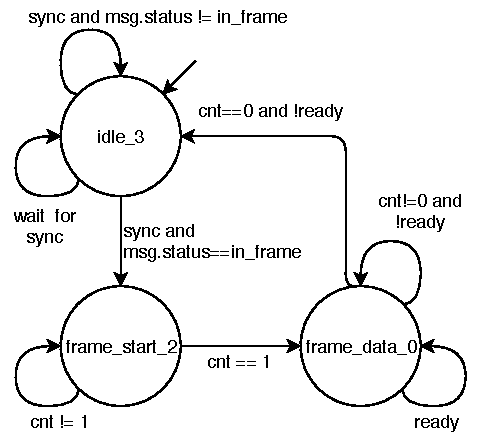
\includegraphics[width=0.25\textwidth]{fig/Example_PPA.pdf}
\end{wrapfigure}

Figure~\ref{fig:example_operation} shows an abstract view of the operation \textit{P2}. 
The assume part shows the trigger conditions.
The assumptions are that the component is in the control state \textit{L17}, there is a new value (\textit{sync $==$ true}) and the message status is \textit{in\_frame}. 
Then, the expectations regarding the component are:
\begin{itemize}
\item transition to state \textit{L.24}
\item the value of the shared port evaluates to \textit{true}
\item the counter is equal to 3
\end{itemize}

\subsubsection{PPA generation}

The result of the previous step is a set of states representing communication calls at the system level and operations describing transitions between states.
The PPA describes a model in terms of its I/O behavior, but the part of the behavior that is implicitly defined by the handshaking of the interfaces is not present in the blockCFG and, thus, is not described by the set of properties yet.
To account for this, the user is only allowed to use the provided interfaces for describing communication, as DeSCAM is completely aware of their underlying handshaking mechanisms.
Each interface implements different handshaking mechanisms, which are added by DeSCAM to the set of properties automatically. 

First, the blockCFG doesn't contain a reset operation.
The \textbf{reset-operation}, is implicitly defined by the C++ semantics of the constructor. 
The ending state is the first communication after reset and the initial values result from the constructor and the path to the first communication.  
The path to the first communication has to be unique. 
Reading from a shared port or master port may result in multiple paths from the reset to the first synchronized communication call. 

The \textbf{wait operation} results from the communication of a blocking port. 
If \textit{read()}\,/\,\textit{write()} is called and the counterpart is not ready, then the module blocks. 
This behavior is implicitly defined through event based handshaking of the interface. 
The implementation is found in \textit{src/Interfaces/}. 
DeSCAM adds a wait operation to the PPA that enforces the module to remain in its state until the counterpart is ready for communication. 

The \textbf{non-blocking-operation} results from the communication of a blocking port and \textit{nb\_read()}\,/\,\textit{nb\_write()} is called. 
The success of the communication is returned by the communication call. 
Here the operation is split into two operations, one for a successful communication and one for the unsuccessful communication.  

\subsubsection{PPA optimization}

Initially, the PPA has four states, one for each communication call. 
Ports with the master interface form a special case, because they do not implement the two-sided handshaking mechanism. 
A distinct state for a master is only required if the port is accessed multiple times in a row without passing a state with synchronization in between. 

For example, if \textit{L.26} evaluates to \textit{false} the state \textit{L.24} is accessed multiple times in a row. 
In order to send the messages (3, 2 and 1 ) in the correct order the hardware remains in state \textit{L.24} and changes the output accordingly. 

For \textit{L.33} this is not the case. 
The successor of \textit{L.33} is either \textit{L.31} or \textit{L.17}. 
A distinct state is not required and the message of \textit{L.33} is send concurrently with the synchronization of \textit{L.31}. 
The state \textit{L.33} is merged with the state \textit{L.31}, this means that the operations L.31$\rightarrow$L.33 and L.33$\rightarrow$L.31\,/\,L.33$\rightarrow$L.17 are merged together to L.31$\rightarrow$L.17 and L.31$\rightarrow$L.31. 
Figure~\ref{fig:example_merge_state} shows the resulting operation for the merge of  L.31$\rightarrow$L.33 and L.33$\rightarrow$L.31.  

\begin{wrapfigure}{r}{0.25\textwidth}
		\centering
			\vspace{-20pt}
		\caption{Merged operation}
		\label{fig:example_merge_state}
		\begin{small}
		\begin{lstlisting}
assume:
 state == L.31 and
 sync == false and 	
 ready == false and
 cnt != 0 
prove: 
 state == L.31
 cnt == cnt-1;
 m_out == msg.data;
\end{lstlisting}
\end{small}
\end{wrapfigure}
 
The resulting PPA is shown in Figure~\ref{fig:example_PPA}. 
In contrast to Figure~\ref{fig:cfg_colored}, DeSCAM names the states not by the line of code they are declared in. 
Instead, states are named by section they are declared and extended by a unique id. 
If there are multiple communication calls within one section they are differentiated by the unique id. 
This is one of the main reasons why we emphasize to use sections as much as possible. 
In absence of sections, a meaningful naming of the states is not possible and states may only be identified by their unique number. 
In our example, \textit{L.17} is renamed to \textit{idle\_3}, \textit{L.24} is renamed to \textit{frame\_start\_2} and \textit{L.33} is renamed to \textit{frame\_data\_0}. The state \textit{frame\_data\_1} is missing because it is merged with \textit{L.31}.

\begin{wrapfigure}{l}{0.3\textwidth}
	\vspace{-20pt}
    \caption{Example blockCFG}
    \label{fig:cfg_colored}
    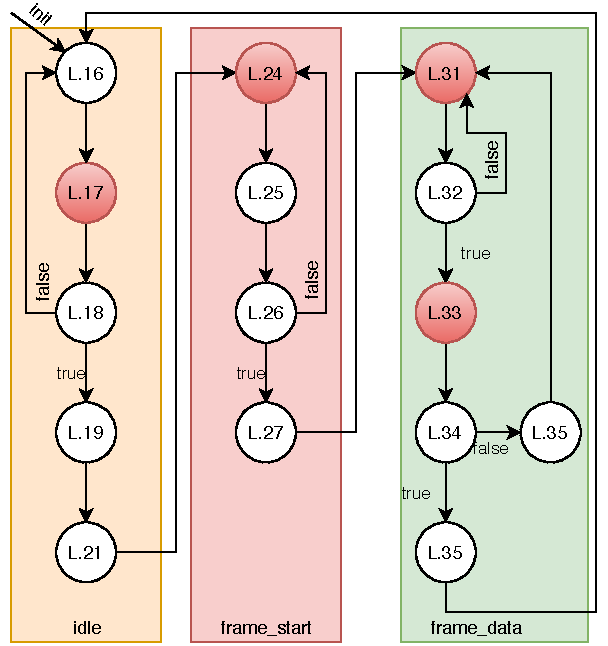
\includegraphics[width=0.3\textwidth]{fig/example_cfg_colored.pdf}
    \vspace{-20pt}
\end{wrapfigure}

Within Figure~\ref{fig:example_PPA} there is an edge for each operation, including the reset. 
The edges show the trigger conditions. For simplicity, the expectations are left out. 
The figure displays the difference between the interfaces. 
The state \textit{idle} has a wait operation in case that the counterpart is not ready for communication whereas the state \textit{frame\_data\_0} doesn't have a wait operation because the communication call uses the non-blocking \textit{nb\_read()} method. 
\textit{Frame\_start} doesn't have any synchronization conditions, because the interface is that of a master.  
The user has the option to generate different views of the PPA in dot format by running DeSCAM with, e.g., -DOTfull or -DOTsimple.  

The last optimization step is the reduction of the number of visible registers. 
At first, each variable at the system level results in a visible register. 
If the variable is only used to store intermediate values, there is no need to latch the value and thus a register bears unnecessary overhead. 

In the given example, this is the case for the variable \textit{ready}, which stores the success of \textit{nb\_read()} at line~31. 
The variable is assigned the value of the success of communication via port \textit{b\_in}. 
The trigger condition resulting from the if-then-else at line~32 is dependent on the evaluation of the communication. 
DeSCAM takes care of this by replacing each occurrence of \textit{ready} with \textit{b\_in\_sync} in each operation leaving \textit{frame\_data\_0}.
Afterwards, it is checked whether the variable is used in any other operation.
Since this is not the case, the variable is not part of the state variables and thus no visible registers is necessary. 
 
For example, the variable \textit{cnt} at line~35 is assigned its previous value decreased by one. 
The new value is dependent on the previous and thus the variable becomes part of the state space of the PPA and a visible register is introduced. 


\textbf{Modules}

Modules that are considered to be a slave module form a special case.
The generated properties ensure that a message from a master is never lost. 
At the system level the interface is implemented using a one-sided handshake.
The master port is blocked until the slave is ready.

In order to model this behavior at the RTL, it is assumed that all slave ports communicate concurrently. 
Therefore, the tool merges sequences of slave communications into a single important state. 
A sequence here describes a path in the PPA where each of the slave ports is accessed exactly once. 
The access order is of importance, it has to be ensured that each sequence accesses the ports in exactly the same order at the system-level. 
Here, the first sequence from reset is the reference for the other sequences.

It is important to remember that the slave out port will lose its message if no master is waiting. 
Furthermore, the sync of the slave in port has always to be taken into consideration. 
It is possible that the slave may read before the master is ready! 

\subsection{Step 2: Property generation}

The PPA is now stored as internal data structure within DeSCAM. 
In order to generate the properties the user runs DeSCAM with the option -ITL or -SVA.
This invokes a call to the respective backend found in \textit{src/Backend}. 
In this section we are going to focus on the ITL property generation, the generation for the SVA properties follows exactly the same idea. 

Before the properties are generated, the operations of the PPA have to be extended by timing and functions that enable connecting the properties to an RTL implementation. 
In order to link the operations of the PPA to an RTL implementation we introduce \textit{macros}.
The designer is able to relate the abstract symbols of the system level to an arbitrary RTL implementation by refining the macros. 

The generated properties are formalized with the macros, which then get replaced by the parser with the according RTL signals.
For example, there is a macro for the variable \textit{cnt} and within the properties \textit{cnt} is referenced by this macro. 
The designer has the task to refine the macro and thereby providing the information how \textit{cnt} is implemented at the RTL. 
Macros are generated for the ports and the handshaking, the visible registers as well as the important states. 

\begin{verbatim} macro MACRO_NAME : RETURN_TYPE := MACRO_BODY end macro; 
\end{verbatim}
For filling the macros there are only three rules:
\begin{itemize}
\setlength\itemsep{0em}
\item Only finite sequences (of arbitrary length) may be evaluated
\item Functions characterizing abstract inputs may be expressions
over only input signals of the RTL design.
\item Functions characterizing abstract outputs may be expressions
over only output signals of the RTL design.
\end{itemize}
The name of the macro and the return type are provided by the tool. 
The designer has the task to refine the macro body according to the implementation.
When SVA properties are generated the macros are exchanged by a function/define, but the idea remains the same. 

\subsubsection{Port Macros}

In general, for each blocking port macros for the notify, sync and datapath are generated. 
For the master interface a sync signal is not necessary and only the \textit{master\_out} port requires a notify signal and thus only the \textit{slave\_in} port requires a sync signal.
The ports of type \textit{shared} and \textit{slave\_in} require no synchronization. 
The datapath signal transports the actual message.

\subsubsection{Visible Registers}

The visible registers are part of the state space of the design. 
There is a visible register for each variable that is used at the system level, if the register is not removed in the previous optimization step. 
The macros for compound types are split into separate macros for each subtype. 
For example, the variable \textit{msg} is separated into two macros \textit{msg\_data} and \textit{msg\_status}.

\subsubsection{Important States}

The important states are derived from the communication calls at the system level. 
In our example we have three important states, \textit{idle\_3}, \textit{frame\_start\_2} and \textit{frame\_data\_0}. 
The important states macros are of a boolean return type.
If the hardware is in an important state the macro should evaluate to \textit{true}, \textit{false} otherwise. 

\subsubsection{Properties}

\begin{wrapfigure}{R}{0.4\textwidth}
	\vspace{-20pt}
	\caption{Reset operation}
	\label{fig:reset_operation}
\begin{verbatim}
property reset is
assume:
	 reset_sequence;
prove:
	 at t: idle_3;
	 at t: cnt = 0;
	 at t: msg_data = 0;
	 at t: msg_status = in_frame;
	 at t: s_out_sig = false;
	 at t: b_in_notify = true;
	 at t: m_out_notify = false;
end property;
\end{verbatim}
\end{wrapfigure}

We are going to split the generated properties into three different kinds of properties: reset 
operations, regular operations and wait operations.

The \textbf{reset operation} is a special operation, as it defines the state of the hardware after reset. 
This is particularly important, because otherwise properties may not cover all possible behavior. 

Let's take a look at the reset property in Figure~\ref{fig:reset_operation} from our example in Figure~\ref{fig:system-c-example-complex}. 
The property is split into two parts: An assume part defining the trigger conditions and an expect part describing the expectations. 

One may read the properties as if-then relation. 
In this case: \textbf{if} \emph{reset\_sequence} \textbf{then} prove that \emph{idle\_3 and cnt=0 and ...}. 
In state idle\_3 the port \textit{b\_in} reads and thus the macro \textit{b\_in\_notify} has to evaluate to \textit{true}. 
At the same time, all other ports are not ready for communication and thus their notify signals have to evaluate to \textit{false}. 


\begin{small}
\begin{wrapfigure}{l}{0.5\textwidth}
	\caption{Regular operation}
	\label{fig:regular_operation}
\begin{verbatim}
property idle_3_read_5 is
dependencies: no_reset;
for timepoints:
	 t_end = t+32;
freeze:
	b_in_sig_data_at_t=b_in_sig_data@t,
	b_in_sig_status_at_t=b_in_sig_status@t;
assume:
	 at t: idle_3;
	 at t: (b_in_sig_status = in_frame);
	 at t: b_in_sync;
prove:
	 at t_end: frame_start_2;
	 at t_end: cnt = 3;
	 at t_end: m_out_sig = 3;
	 at t_end: msg_data=b_in_sig_data_at_t;
	 at t_end: msg_status=b_in_sig_status_at_t;
	 at t_end: s_out_sig=true;
	 during[t+1, t_end]: b_in_notify = false;
	 during[t+1, t_end-1]: m_out_notify = false;
	 at t_end: m_out_notify = true;
end property;\end{verbatim}

\end{wrapfigure}
\end{small}

The next property to look at is a regular \textbf{operation} as shown in Figure~\ref{fig:regular_operation}. 
This operation describes the path from line~17 to line~24 in the code. 
A value from port \textit{b\_in} is read and afterwards the port \textit{m\_out} writes the first value. 
This path is only taken if the condition at line~18 evaluates to \textit{true}. 
The evaluation of this condition is dependend on the value read from port \textit{b\_in}. 

The property is segmented into different parts. 
It starts with the dependencies, all we need is to assume that there is no reset, but the designer may add additional environment constrains to the properties. 
The next segment allows the designer to specify the length of an operation in number of clock cycles. 
The time point \textit{t\_end} specifies when the prove part should be evaluated. 
The default value is set to \textit{t+1}. 
In this case the property uses \textit{t+32}. 
Besides the constraints, the designer is only allowed to change the value of \textit{t\_end}. 
Everything else in the property has to remain untouched. 
Changing the properties in any other way may result in a loss of completeness!

Next, the values of the input signals are frozen at \textit{t}, this means that the value of the signal is stored in a variable at time point \textit{t}. 
In general, all values of the inputs and variables are captured at time point \textit{t}, while the values of the outputs are set at time point \textit{t\_end}. 

The assume part specifies the assumptions (trigger conditions), which are all evaluated at time point \textit{t}. 
The first condition is that hardware is in state \textit{idle\_3}, which means that the port \textit{b\_in} waits for a new message.
The operation is only triggered if a new message is available and the \textit{b\_in\_sync} macro evaluates to \textit{true}. 
The case that there is no new message is covered by the respective wait operation.
The last condition of the assume part is more interesting, because it differentiates from what the designer may expect by looking at the SystemC-PPA. 
The condition results from line~18. The condition is not described using the variable \textit{msg.status}, instead the evaluation of the condition is based on the macro \textit{b\_in\_sig\_status}. 
At the system level the value of a variable changes instantly upon assignment. 
At the RTL the value of a register changes with the next clock event. 
In order to evaluate the condition upon handshake completion, the value of the input signal has to be evaluated. 
DeSCAM propagates the input signals through the paths. 

\begin{wrapfigure}{r}{0.5\textwidth}
	\vspace{-20pt}
	\caption{Wait operation}
\begin{verbatim}
property wait_idle_3 is
dependencies: no_reset;
freeze:
	cnt_at_t = cnt@t,
	msg_data_at_t = msg_data@t,
	msg_status_at_t = msg_status@t,
	s_out_sig_at_t = s_out_sig@t;
assume:
	 at t: idle_3;
	 at t: not(b_in_sync);
prove:
	 at t+1: idle_3;
	 at t+1: cnt = cnt_at_t;
	 at t+1: msg_data = msg_data_at_t;
	 at t+1: msg_status = msg_status_at_t;
	 at t+1: s_out_sig = s_out_sig_at_t;
	 at t+1: b_in_notify = true;
	 at t+1: m_out_notify = false;
end property;
\end{verbatim}
\end{wrapfigure}

The last segment is \textit{prove}, which defines the next state of the hardware. 
All changes of the state variables and outputs are proven at time point \textit{t\_end}. 
In this case the hardware transitions from state \textit{idle\_3} to \textit{frame\_start\_2} and the signal \textit{cnt} takes the value 3.
The variable \textit{msg} stores the message, which is frozen at time point \textit{t} in the freeze-variables \textit{b\_in\_sig\_data\_at\_t} and \textit{b\_in\_sig\_status\_at\_t}. 
The registers are updated to the value of \textit{b\_in} at \textit{t} not at \textit{t\_end}. 
As mentioned earlier, outputs are set at \textit{t\_end} whereas inputs are read at \textit{t}. 

A \textbf{wait operation} is generated for each blocking message transfer. 
There are only two assumptions for a wait operation: The hardware in a specific state and the respective sync signal is low. 
Then it is proven, that that hardware remains in the same state.
Thus the state variables, outputs and the important states have to remain the same. 
Furthermore, the property is only one cycle long.
This is due to fact that the respective port already offers a handshake and an incoming sync should not be missed. 
This property stays entirely unchanged within the refinement process. 

A special case are the \textbf{slave modules}. 
Here, all generated properties are forced to be exactly one cycle long and thus ( due to the state merging) every slave communicates once in each clock cycle and is always ready for its master port. 


\subsection{Step 3: Implementation and Refinement}
\begin{wrapfigure}{l}{0.5\textwidth}
	\vspace{-20pt}
    \caption{Implementation process}
    \label{fig:step3_detail}
    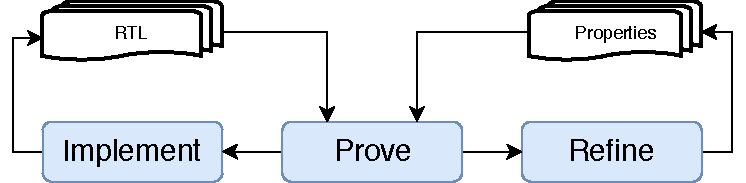
\includegraphics[width=0.5\textwidth]{fig/step3_detail.pdf}
    \vspace{-20pt}
\end{wrapfigure}

The last step of the PDD methodolgy is the implementation of the hardware and the refinement of the properties. 
As an example, we use the design of Figure~\ref{fig:system-c-example-complex}, which is considered to be the golden model for the hardware design process. 
Figure~\ref{fig:step3_detail} provides an overview of the desired flow, which consist of three major steps: refinement, implementation and proof. 
An iteration of the flow starts with choosing a property to implement, implementing the property and in parallel refining the properties accordingly. 
If the chosen property holds on the design, the flow starts from the beginning. 
 
The minimum requirements for the first iteration of the flow are an RTL template implementation, a set of properties and a property checker. 
The template has to implement the desired I/O interface, but is not required to have any behavioral elements. 
The macros for ports and visible registers of the set of properties have to be refined according to the RTL template.  
Finally, the template and the properties are loaded with a property checker. 
The first property that should be implemented is the \textit{reset property} and the implementation and properties are refined such that the reset property holds.  

As the last step in every iteration, the property checker examines whether the considered property holds on the design. 
It thereby proves whether the hardware is correctly implemented for this property. 
If the property holds, the designer should check whether all previously implemented properties still hold. 
If this the case, then, the next property is implemented.
Otherwise, the designer uses the information from the debugger to either change the hardware implementation or to refine the properties.
This depends on whether the counter example is a \textit{false negative} or a \textit{true negative}. 

Generally it is recommendable to begin with implementing all properties that start in the important state after reset. 
Then, all properties from the state after reset are implemented. 
The process continues until all properties hold on the design. 

\subsubsection{RTL template}

In order to start the PDD flow the designer has to provide an RTL template implementation, either in form of an already existing implementation, a custom RTL template or a template generated by DeSCAM.
By running \textit{DeSCAM} with parameter \textit{-VHDL} a structural description of the module is created.
There is a port for each port at the system level transporting the message, ports for synchronization (\textit{sync} and \textit{notify}) and signals for the visible registers. 
The template doesn't have any behavioral elements, although it provides a reset sequence that works with the reset from the properties. 
The designer is free to change anything in this template to his/her convenience. 

The generated template also provides a package containing the declarations of data types used on the system level. 
These types are also used in the properties. 
Hence, if the designer decides to have a manual type declaration it is his/her responsibility to provide these to the property template. 
For example, an \textit{enum} type declared at the system level is represented by the symbolic values of this \textit{enum} type within the properties. 
This largely increases the readability of the properties. 
If the designer decides to implement the \textit{enum} type manually, there has to be a mapping to the symbolic type of the system level.    

We explain, via example, how the abstract ports at the system level are mapped to an arbitrary RTL implementation.
The generated template from the golden reference has a port declaration \textit{b\_in} that transports a message of type \textit{msg\_t}. 
This port provides the message as a 32-bit integer for \textit{msg.data} and a 1-bit boolean for \textit{msg.status}. 

It is assumed that the entire message is not provided by a 33-bit input port. 
Instead, there is a 1-bit input receiving the message sequentially over multiple clock cycles.
The RTL template is adjusted to this new environment by exchanging \textit{b\_in} with a port that provides only a 1-bit input \textit{data\_in}.

These are manual design decisions that are abstracted at the system level. 
The generated properties are based on the abstract objects of the system level. 
The designer has to specify how these objects are implemented at the RTL by refining the properties accordingly. 

\subsubsection{Port and Visible Register Refinement}

After creating the RTL template the properties have to be refined according to this template. 
Initially, the macro bodies of the generated properties are empty and the designer has to refine the macros according to the RTL design. 
For refining the macros three cases are possible, as shown in \textit{Paper.vhi}:
\newpage
\begin{enumerate}
\setlength\itemsep{0em}
\item The macro is not required, because an RTL component with the same name exists and the macro is removed (e.g., line~1\,-\,4). 
\item The macro is required, the RTL signal has a different name (e.g., line~41)
\item The macro is required, the value of the macros evaluates over an arbitrary length or conditions (e.g., line ~19\,-\,30). 
\end{enumerate}

As an example, the macros \textit{b\_in.data} and \textit{b\_in.status}, describing the incoming message, are refined. 
The macro \textit{b\_in\_sig\_data} describes the transmission of the data part of the abstract message. 
These two macros demonstrate the strength of the PDD methodolgy, because the cycle- and bit-abstract exchange of a message at the system level is transformed into a cycle- and bit-accurate implementation. 
The fact that the message is transported sequentially by a 1-bit port is unknown at the system level. 
This is a manual RTL design decision and is a picture perfect example why automatic synthesis from the ESL to RTL is not always feasible.
 
The following section describes, the underlying hardware implementing the transmission and afterwards the refinement of the macro is explained.
The behavioral part of the RTL design (\textit{Paper.vhdl}) is split into two processes. 
The process \textit{control} (line~40 to line~128) implements the automaton described by the PPA and the process \textit{data\_buffer} (line~128 to line~140) implements the buffering of the input stream of \textit{data\_in}. 
The protocol for a message transmission over the sequential port \textit{data\_in} is: 
The hardware is in the important state \textit{idle\_3} and the abstract port \textit{b\_in} waits for a new message  (outgoing \textit{b\_in\_notify} evaluates to \textit{true}). 
A new transmission is started, if the corresponding counterpart sends a new message (incoming \textit{b\_in\_sync} evaluates to \textit{true}).
Now, for 32 clock cycles, the 1-bit values of \textit{data\_in} are buffered. 
The first bit is buffered along with the start of the transmission, indicated by \textit{b\_in\_sync} evaluating to \textit{true}.

Note that the designer is dealing with incomplete implementations during the top-down design process.
The assumed current state of the design process is: The reset property holds and the first operation to implement is \textit{idle\_3\_read\_5} (here implemented by line~56 to line~76). 
In order to implement the operation, the designer starts with the trigger conditions. 
The hardware has to be in the important state \textit{idle\_3} and the incoming \textit{sync} is \textit{true}.  
In \textit{idle\_3} the counter \textit{buffer\_cnt} is initially 0 and starts counting upon transmission start. 
The transmission is finished if the counter reaches the value 31 and thus 32 values of \textit{data\_in} are buffered.
The designer has to implement the expectations of the property, e.g., the visible register \textit{msg\_data} has to store the received message. 

Here, an abstract view on this operation is provided, which is always implicitly given by a property. 
The transmission starts at time point \textit{t} and the first value latched into the buffer is the value of \textit{data\_in} at \textit{t} and the last value is the value of \textit{data\_in} at \textit{t+31}. 
This sums up to total 32 1-bit values at which part the transmission is over and the expectation part of the property is checked. 
The expectations part of the properties specifies that after 32 clock cycles \textit{msg\_data} has the value of \textit{b\_in\_sig\_data} at \textit{t}. 

Now, we assume that the implementation step for this operation is done and the correctness of the implementation is to be checked. 
In order to do so, it is required to refine the behavior of the hardware within the properties. 
Let's take a look at line~9 to line~17 in \textit{Paper.vhi}. 
Here the buffering behavior of the input port is described. 

Eventually, the macro has to return the 32-bit integer from the system level, but in reality the message is composed of 32 1-bit values provided by \textit{data\_in}. 
Thus, the macro is described by a concatenation of values from \textit{data\_in} at different time points. 
Since the value of \textit{b\_in\_sig\_data} is captured at \textit{t}, we need to look into the future in order to describe the upcoming values of \textit{data\_in}. 
ITL provides a \textit{next} operation that enables to look an arbitrary amount of cycles into the future. 
The MSB of the integer is the value of \textit{data\_in} at \textit{t} and the LSB is the value of \textit{data\_in} at \textit{t+31}.

Next, we take a look at the second part of the message, the status bit described by the macro \textit{b\_in\_status} (line~19 to line~31).
At the system level, this information is transmitted as a 1-bit input upon handshake completion.
At the RTL it is implemented over a sequence of time and thus the properties have to describe the RTL behavior in order to link the abstract system-level objects in the properties to the concrete implementation. 

The protocol for the status bit is: The value is dependent on the last four input bits of \textit{data\_in}.
If the sequence is equal to \textit{'1111'}, then the status bit evaluates to \textit{in\_frame} and \textit{oof\_frame} otherwise. 

Within the macro body an ITL method \textit{prev()} is used that allows to look into the past. 
The latching of the values of \textit{data\_in} starts after the reset. 
If there is a reset within the last four cycles, then the macro is only dependent on the values received after the reset. 
For example line~22 describes the case that there is a reset at \textit{t-2}. 
The buffering starts after the reset and thus the only value of \textit{data\_in} that is latched is the value at \textit{t-1}. 
Line~29 is the general case without a reset. 

At this point, we advise the reader to change these macros and elaborate on the counter examples. 
Initially, debugging the counter example is confusing because it is an unusual view on the hardware design process. 
The question the designer has to answer is: ``\textit{Are my properties wrong or my hardware?}".  
The easiest way, to elaborate on this is to follow what the hardware is doing for the provided trace. 
This answers the question on \textit{false} or \textit{true} negative quickly. 

\subsubsection{Important State refinement} 

In this section, a basic idea on the refinement process for important states is provided which specifies which state bits of the global state vector describe the important state. 
In general, the designer is free to describe the important states to his/her convenience. 
Within the scope of our experiments two approaches showed the best results:

\begin{itemize}
\item\textit{Output-based refinement:} 
The notify macros are used in order to describe the current state. 
Each important state implements a communication and thus notify signals are set/unset. 
This enables describing the important state with a one-hot encoding of the notify signals. 
If there are multiple system-level communication calls to the same port the encoding is extended by additional conditions in order to distinguish between these calls. 
\item\textit{State-based refinement:}
The important state is described only dependent on internal state variables. 
\end{itemize}

In the following, the state-based refinement is explained by an example for \textit{idle\_3}.
The presented approach works well if the designer sticks to the best practice recommendation of having a distinct section for each communication.
As mentioned earlier, the implementation starts with an RTL template provided by DeSCAM. 
This template provides a section signal which can be used to distinguish the important states. 

Initially, the macro \textit{idle\_3} is refined with \textit{section=idle}. 
But this leads to a counter example, where \textit{buffer\_cnt} is not zero upon transmission start. 
This is a \textit{false} counterexample, because this state is unreachable from reset. 
The macro is extended to ``\textit{section=idle and buffer\_cnt=0}" in order to start from a reachable state. 

\subsubsection{Timing}
Initially, all operations are assumed to be one cycle long and \textit{t\_end} is defined with \textit{t+1} per default.
In our example, the operations that implement the transmission of the message are actually 32 cycles long. 
The designer has to provide this information by changing \textit{t\_end} to \textit{t+32}. 